\documentclass[10pt]{article}
\usepackage[margin=0.72in]{geometry}
\usepackage{graphicx}
\usepackage{booktabs}
\usepackage{amsmath}
\usepackage{enumitem}
\usepackage{hyperref}
\usepackage{float}
\setlength{\parskip}{0.35em}
\setlength{\parindent}{0pt}

\title{\textbf{Big Data Cup 2026 (Rough Draft v1)}\\Off-Puck Space Creation Value}
\author{Working Draft}
\date{February 2026}

\begin{document}
\maketitle
\vspace{-1.1em}

\textbf{Question.} Which players and teams create offensive value \emph{without} puck touches by moving defenders, opening seams, and increasing shot opportunity quality?

\textbf{Data + scope.} 10 games from the public BDC 2026 release, 5v5 only. We segment 4{,}257 offensive-zone possessions and evaluate 83{,}149 off-puck frame contributions (frame stride = 25).

\section*{1. Approach Summary}
For each sampled frame in an offensive possession:
\begin{itemize}[leftmargin=1.2em,itemsep=0.2em]
    \item Build an \textbf{Opportunity Field} from (i) slot openness, (ii) seam openness, and (iii) shooter release space.
    \item Attribute each non-carrier skater's impact with a leave-one-out freeze:
    \[
    \Delta O_t^{(A)} = O_t(\text{all}) - O_t(\text{player A frozen at prior position}).
    \]
    \item Define \textbf{Space Creation Added (SCA)} as summed/averaged $\Delta O_t$ over off-puck windows.
    \item Detect off-puck action tags (cut, drag, screen, decoy) with rule-based motion/location logic.
\end{itemize}

\textbf{Validation targets.} Primary target: possession ends in shot/goal. Secondary: slot shot/goal.

\begin{figure}[H]
    \centering
    \begin{minipage}[t]{0.49\textwidth}
        \centering
        
\includegraphics[width=\textwidth]{figures/fig_model_auc.png}
    \end{minipage}
    \hfill
    \begin{minipage}[t]{0.49\textwidth}
        \centering
        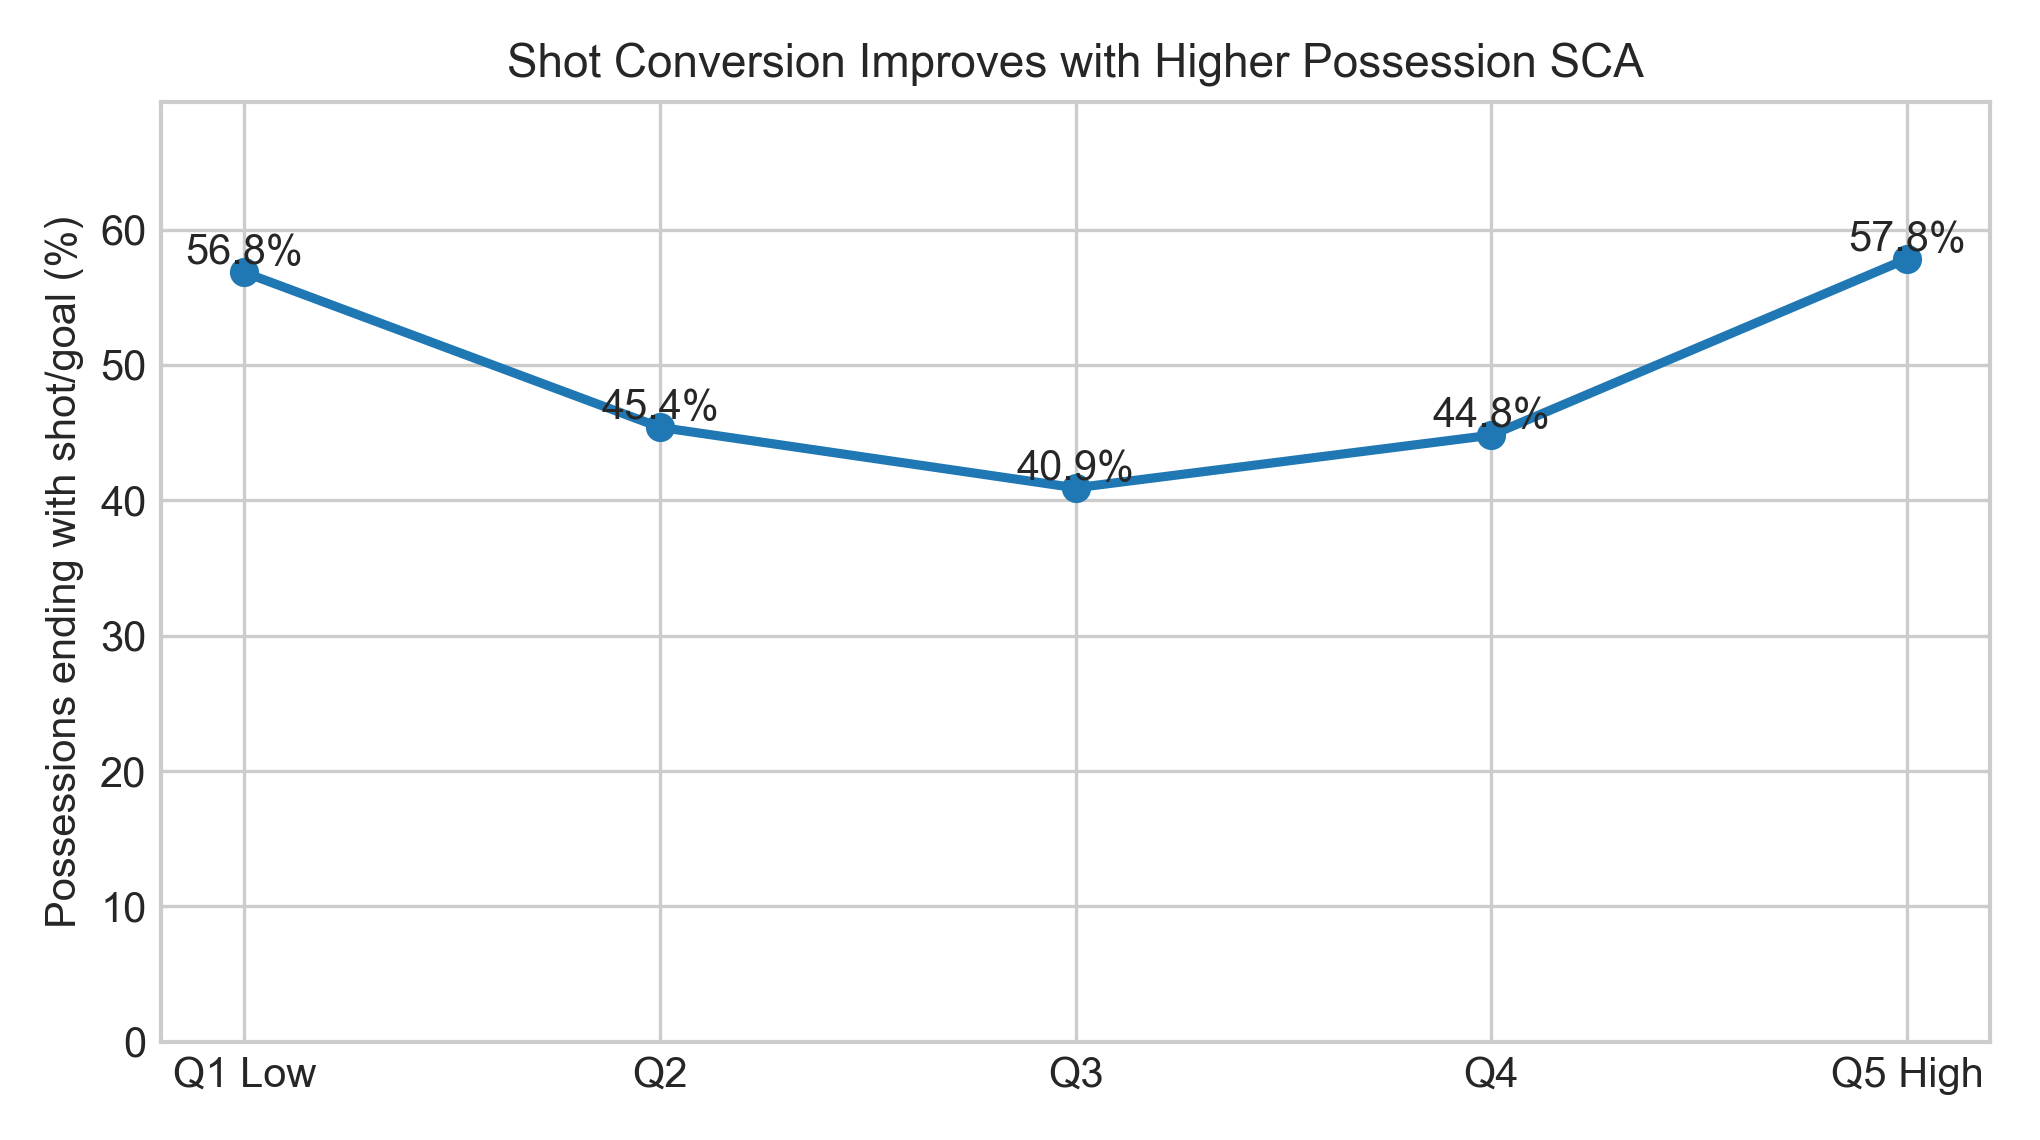
\includegraphics[width=\textwidth]{figures/fig_possession_quintiles.png}
    \end{minipage}
    \caption{Left: SCA adds signal on top of possession duration for shot prediction. Right: shot rates by possession SCA quintile (descriptive, unadjusted).}
    \label{fig:model_quintile}
\end{figure}

\section*{2. Core Findings}
\textbf{SCA adds incremental predictive value.}
\begin{itemize}[leftmargin=1.2em,itemsep=0.2em]
    \item Duration-only model: AUC $=0.705\pm0.010$.
    \item SCA-only signature: AUC $=0.643\pm0.010$.
    \item Duration + SCA: AUC $=0.717\pm0.007$.
\end{itemize}
Interpretation: off-puck features are not a replacement for possession length/context, but they provide additive signal.

\textbf{Archetypes emerge from movement style.}
Clustering identifies at least four robust archetypes: low-activity fillers, drag/cut seam manipulators, screen-dominant net-front players, and balanced support movers.

\textbf{Action-level effect estimates.}
In this baseline model, drag and cut actions show positive mean lift on opportunity, while screen/decoy flags are negative on average (likely because many occur in already-crowded late-phase possessions).

\begin{figure}[H]
    \centering
    \begin{minipage}[t]{0.49\textwidth}
        \centering
        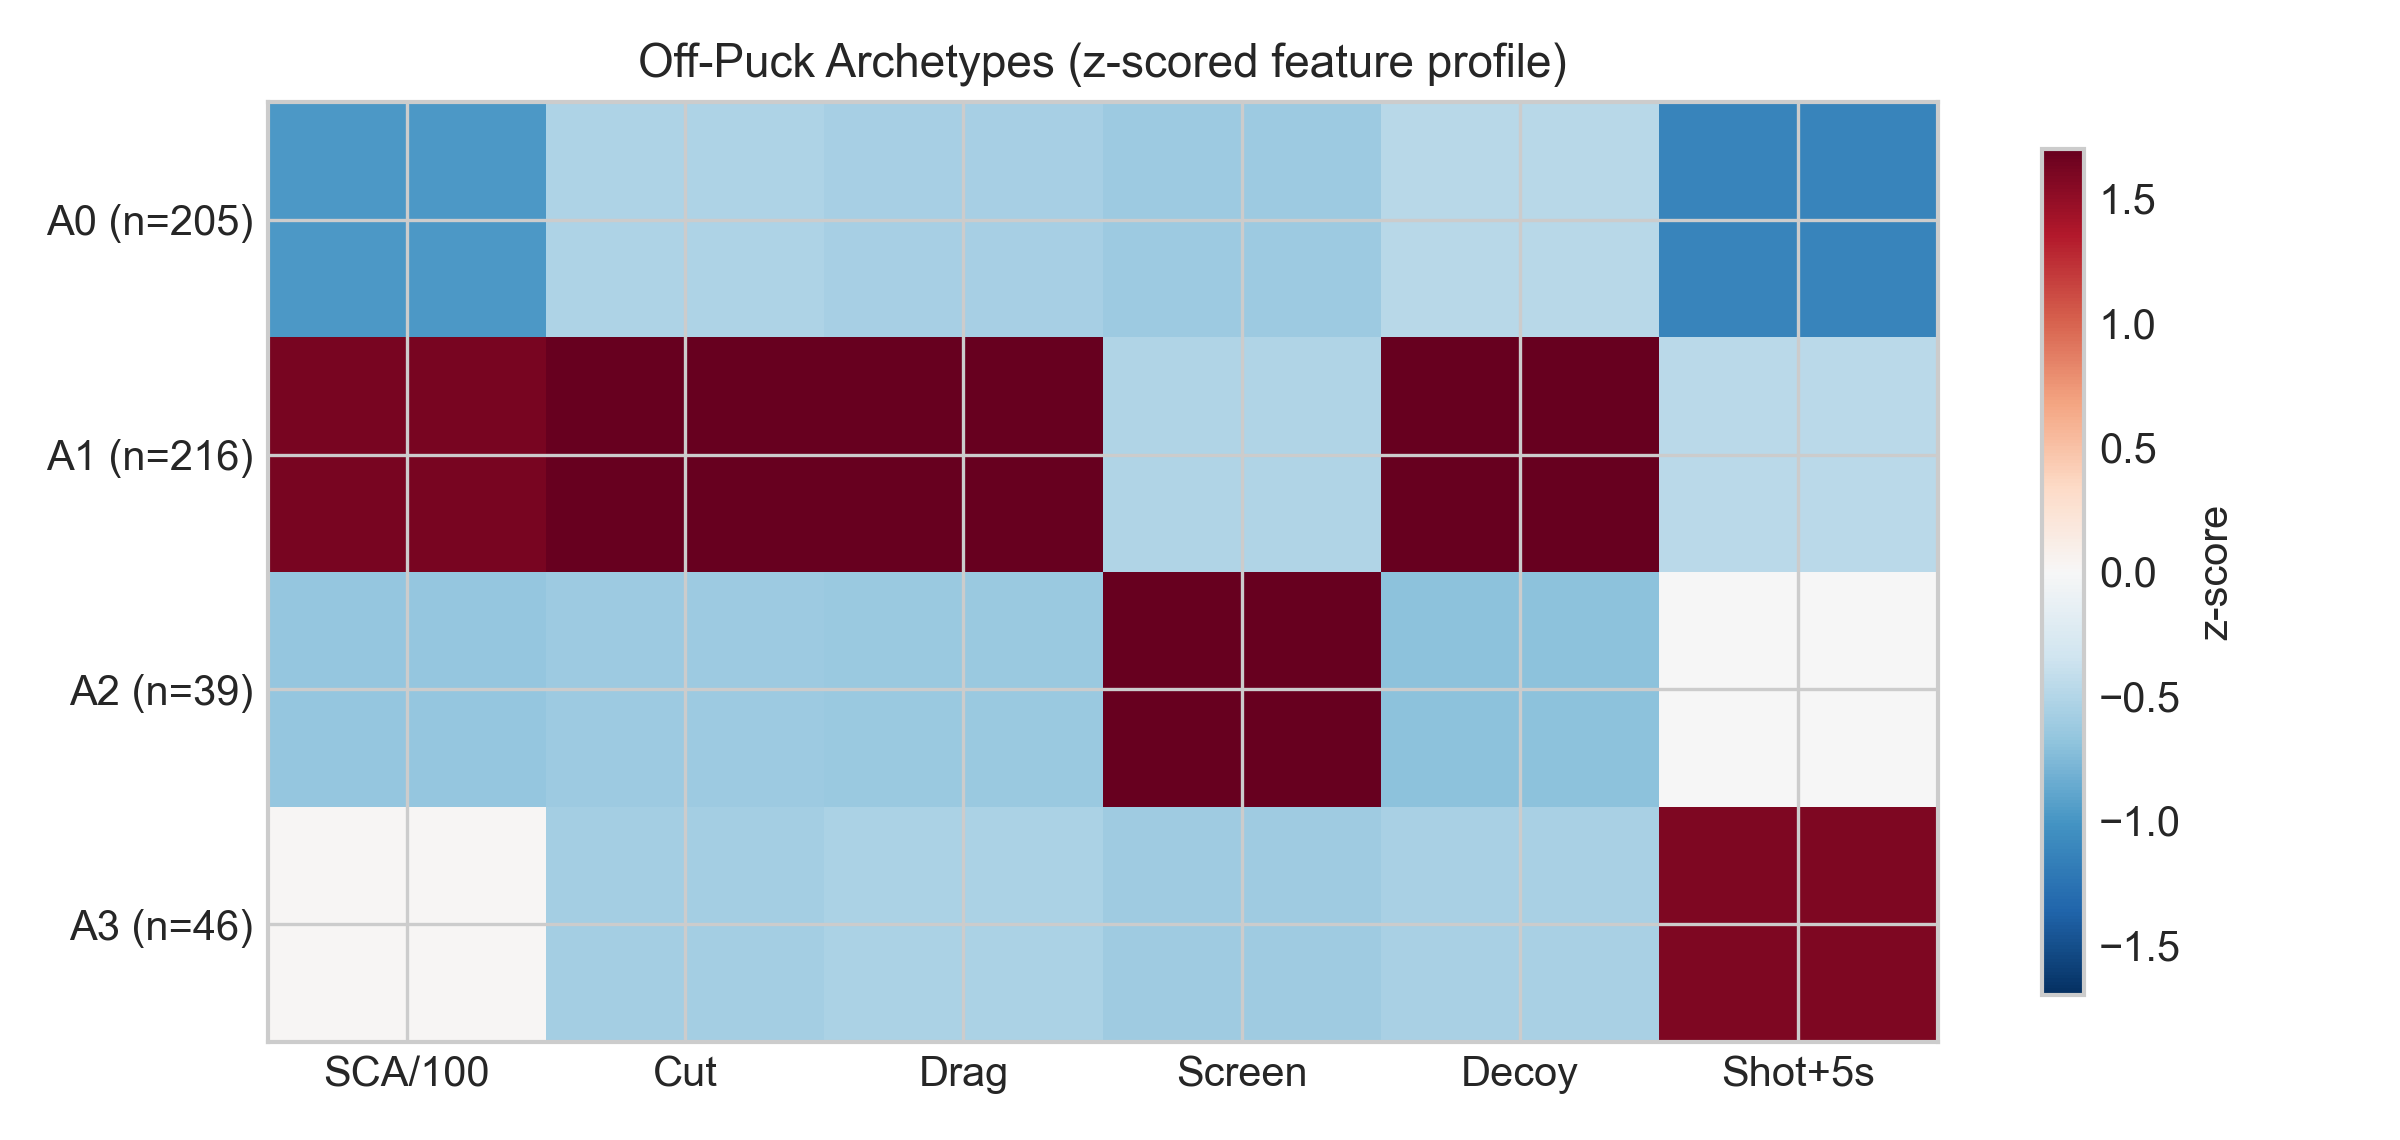
\includegraphics[width=\textwidth]{figures/fig_archetype_heatmap.png}
    \end{minipage}
    \hfill
    \begin{minipage}[t]{0.49\textwidth}
        \centering
        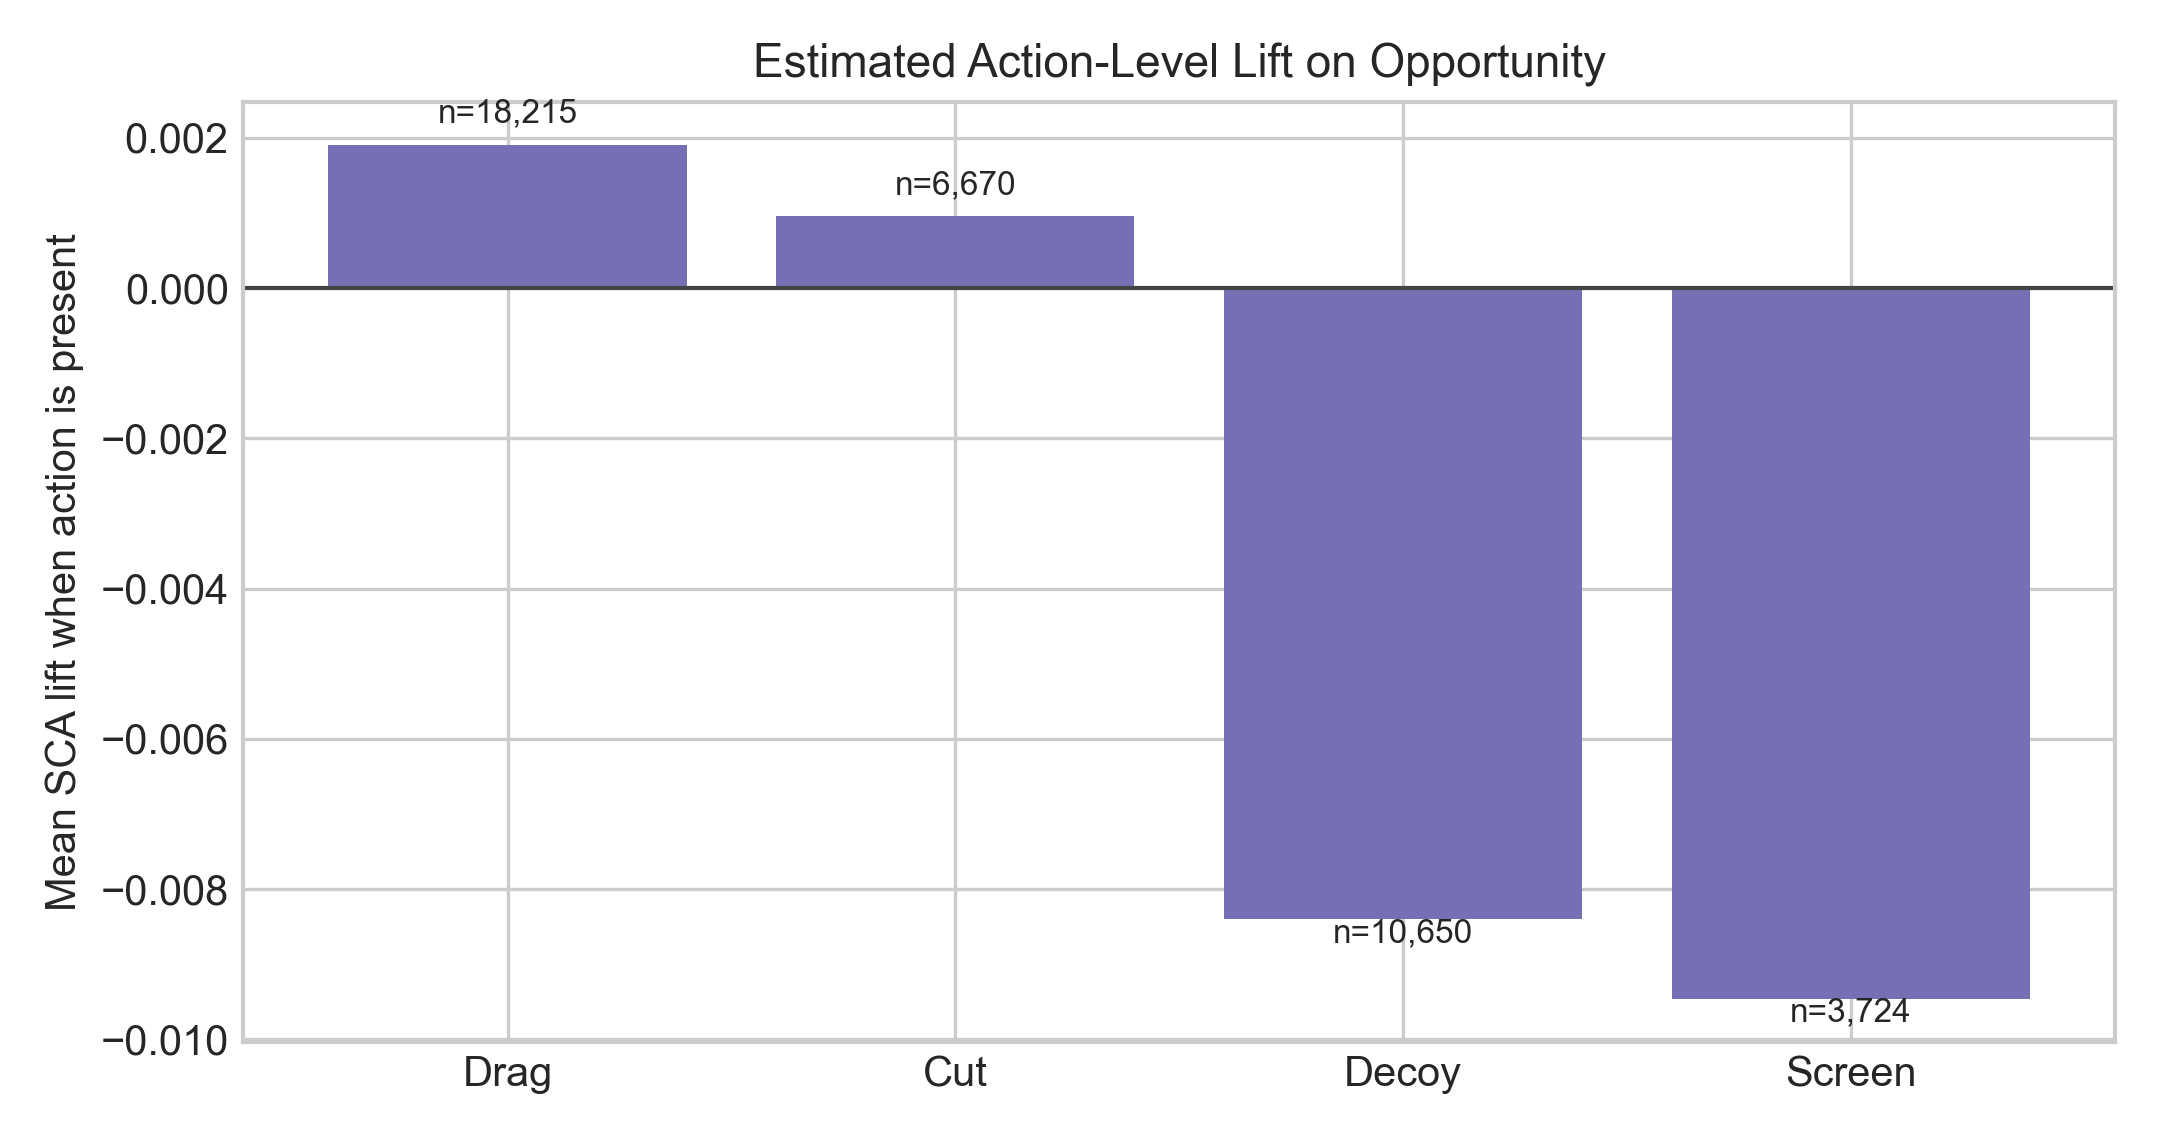
\includegraphics[width=\textwidth]{figures/fig_action_lift.png}
    \end{minipage}
    \caption{Left: z-scored archetype feature profiles. Right: estimated action lift on frame-level opportunity.}
    \label{fig:arch_action}
\end{figure}

\section*{3. Actionable Recommendations (GM / Head Coach)}
\textbf{A. Track SCA as a complementary KPI, not a standalone score.}
Use SCA alongside zone time and quality-of-opposition controls. Deployment decisions should combine all three.

\textbf{B. Prioritize drag/cut movement patterns in O-zone structure work.}
The strongest positive lifts come from lateral manipulation and slot-attacking cuts; build drills around coordinated off-puck lane swaps and timing.

\textbf{C. Use player archetypes for roster construction and line fit.}
Balance line trios with at least one high drag/cut manipulator and one stabilizer; avoid stacking low-activity archetypes in top-six usage.

\textbf{D. Add team-level SCA benchmarking to pre-scout.}
Current sample suggests strong positive mean possession SCA for Team E / Team I, with negative means for Team L / Team F, indicating different defensive attention burdens to prepare for.

\begin{figure}[H]
    \centering
    \begin{minipage}[t]{0.49\textwidth}
        \centering
        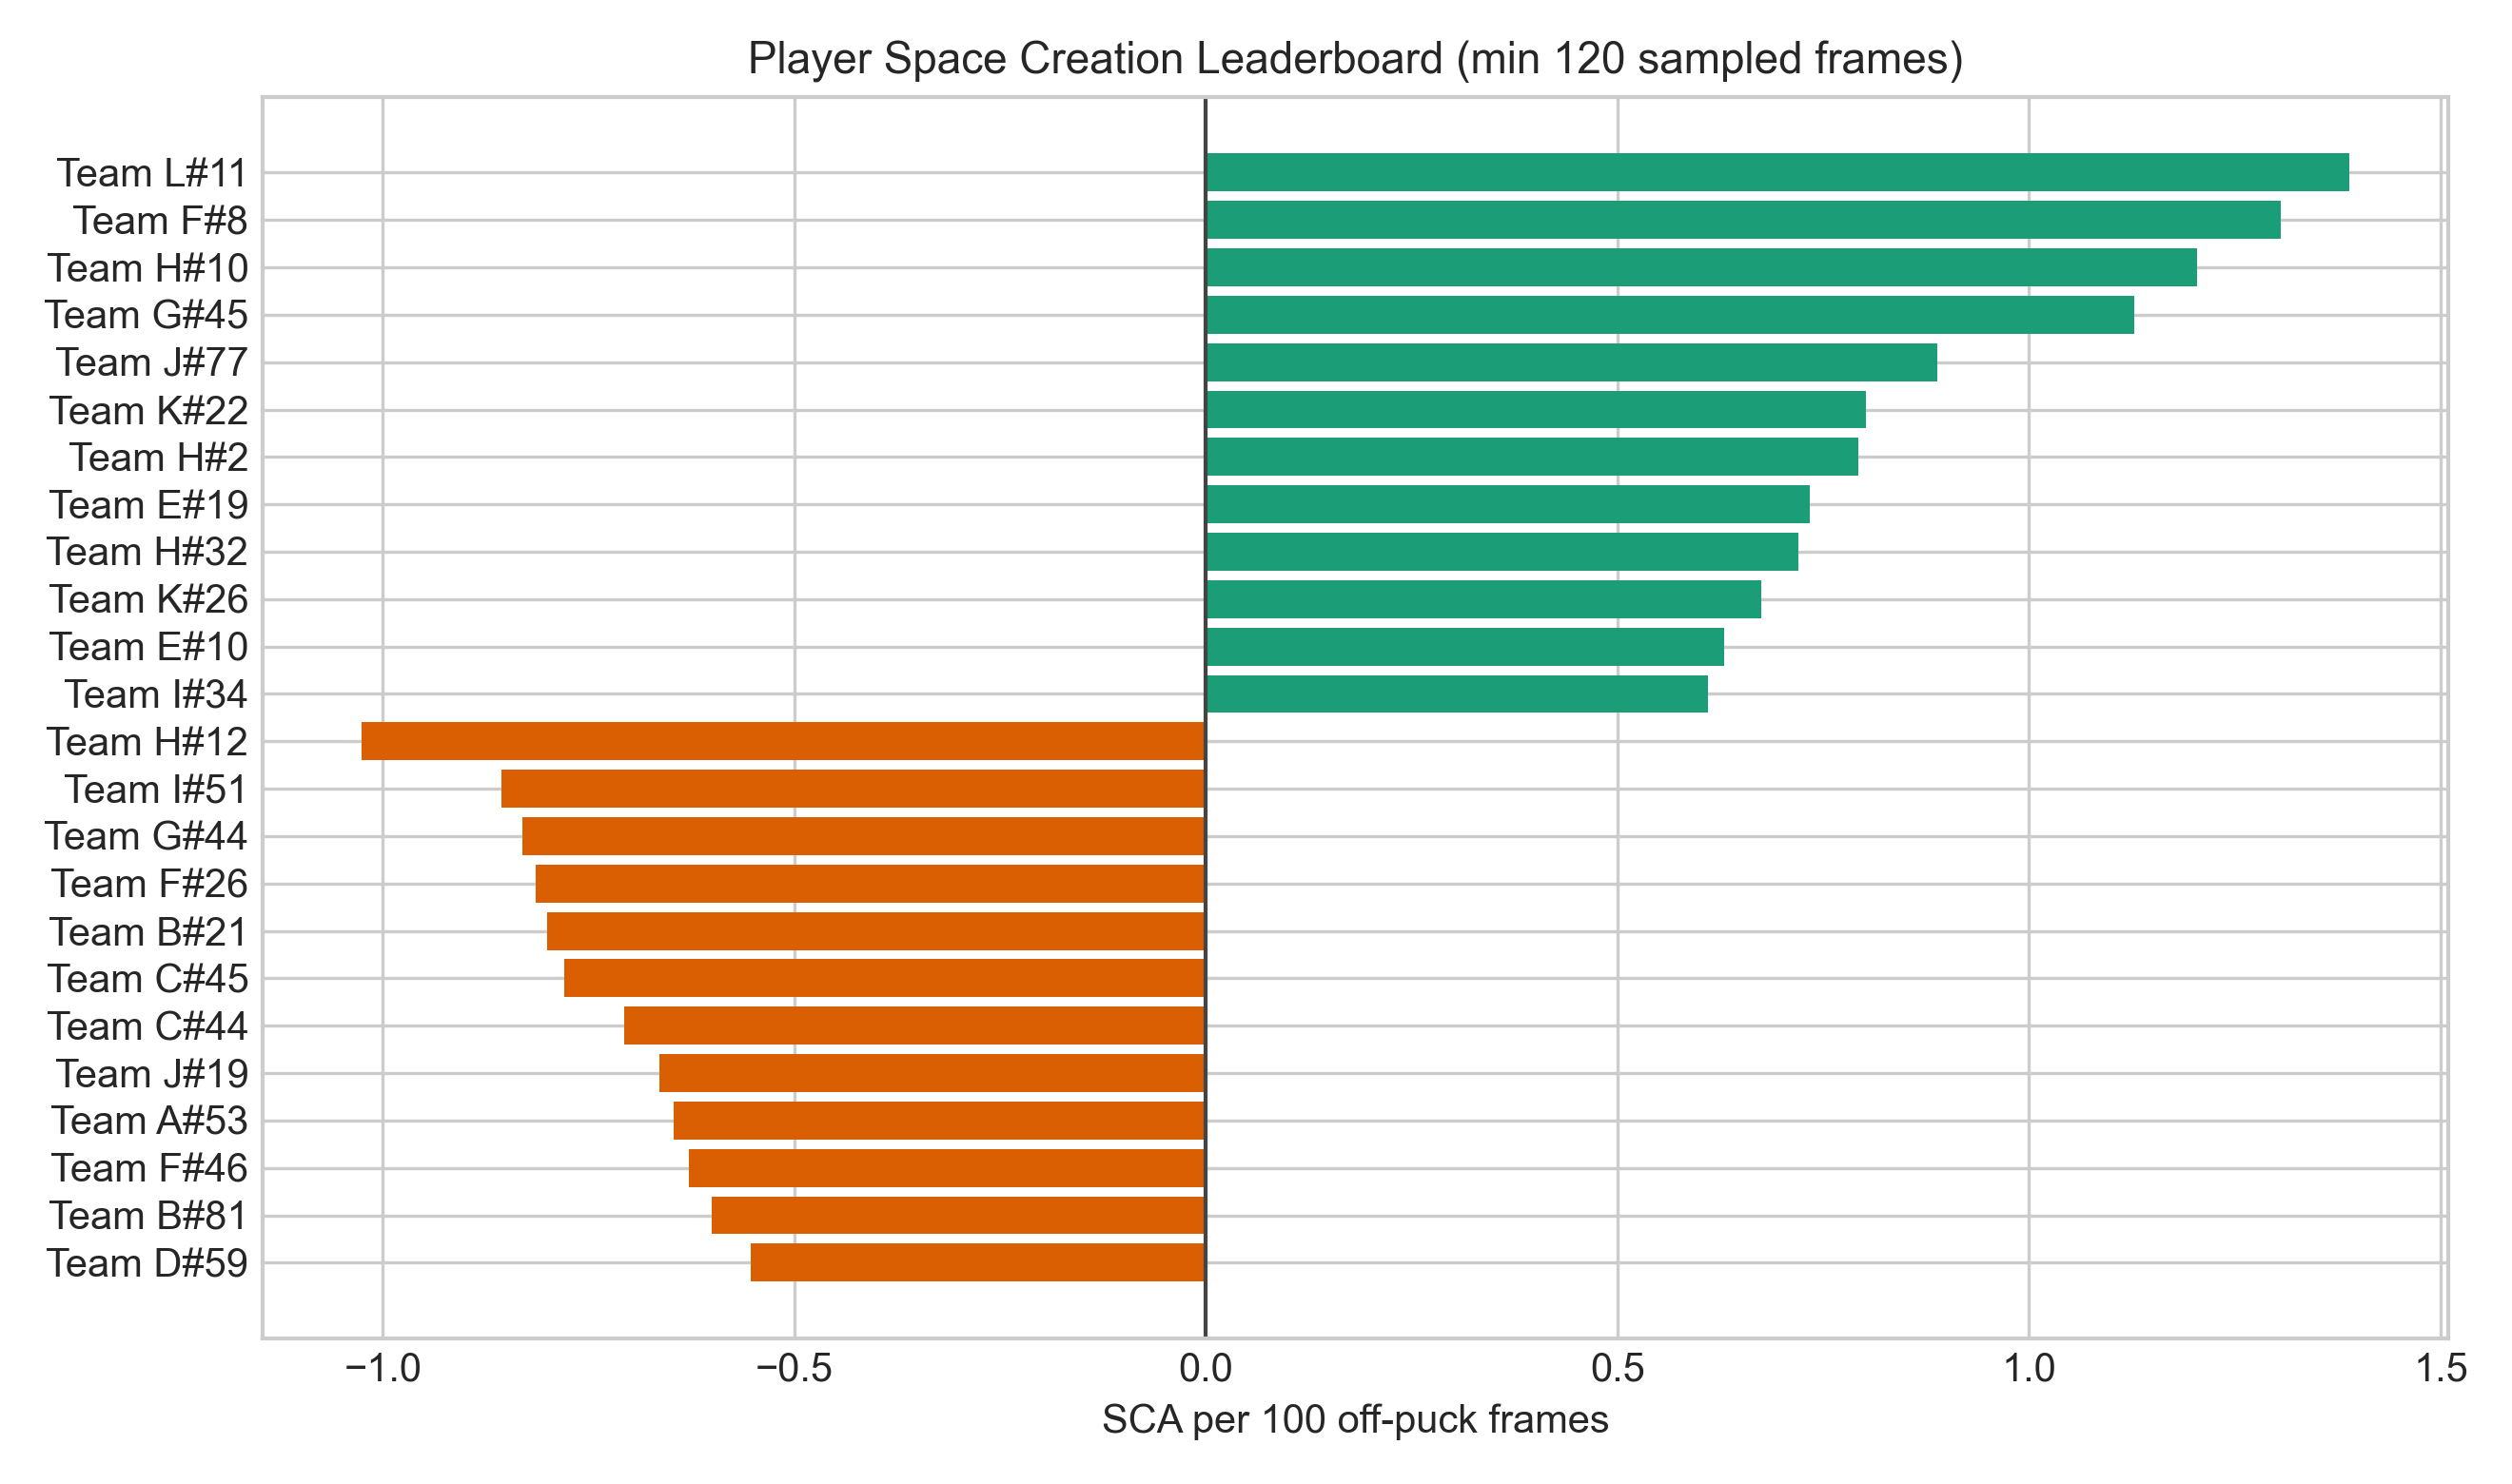
\includegraphics[width=\textwidth]{figures/fig_player_leaderboard.png}
    \end{minipage}
    \hfill
    \begin{minipage}[t]{0.49\textwidth}
        \centering
        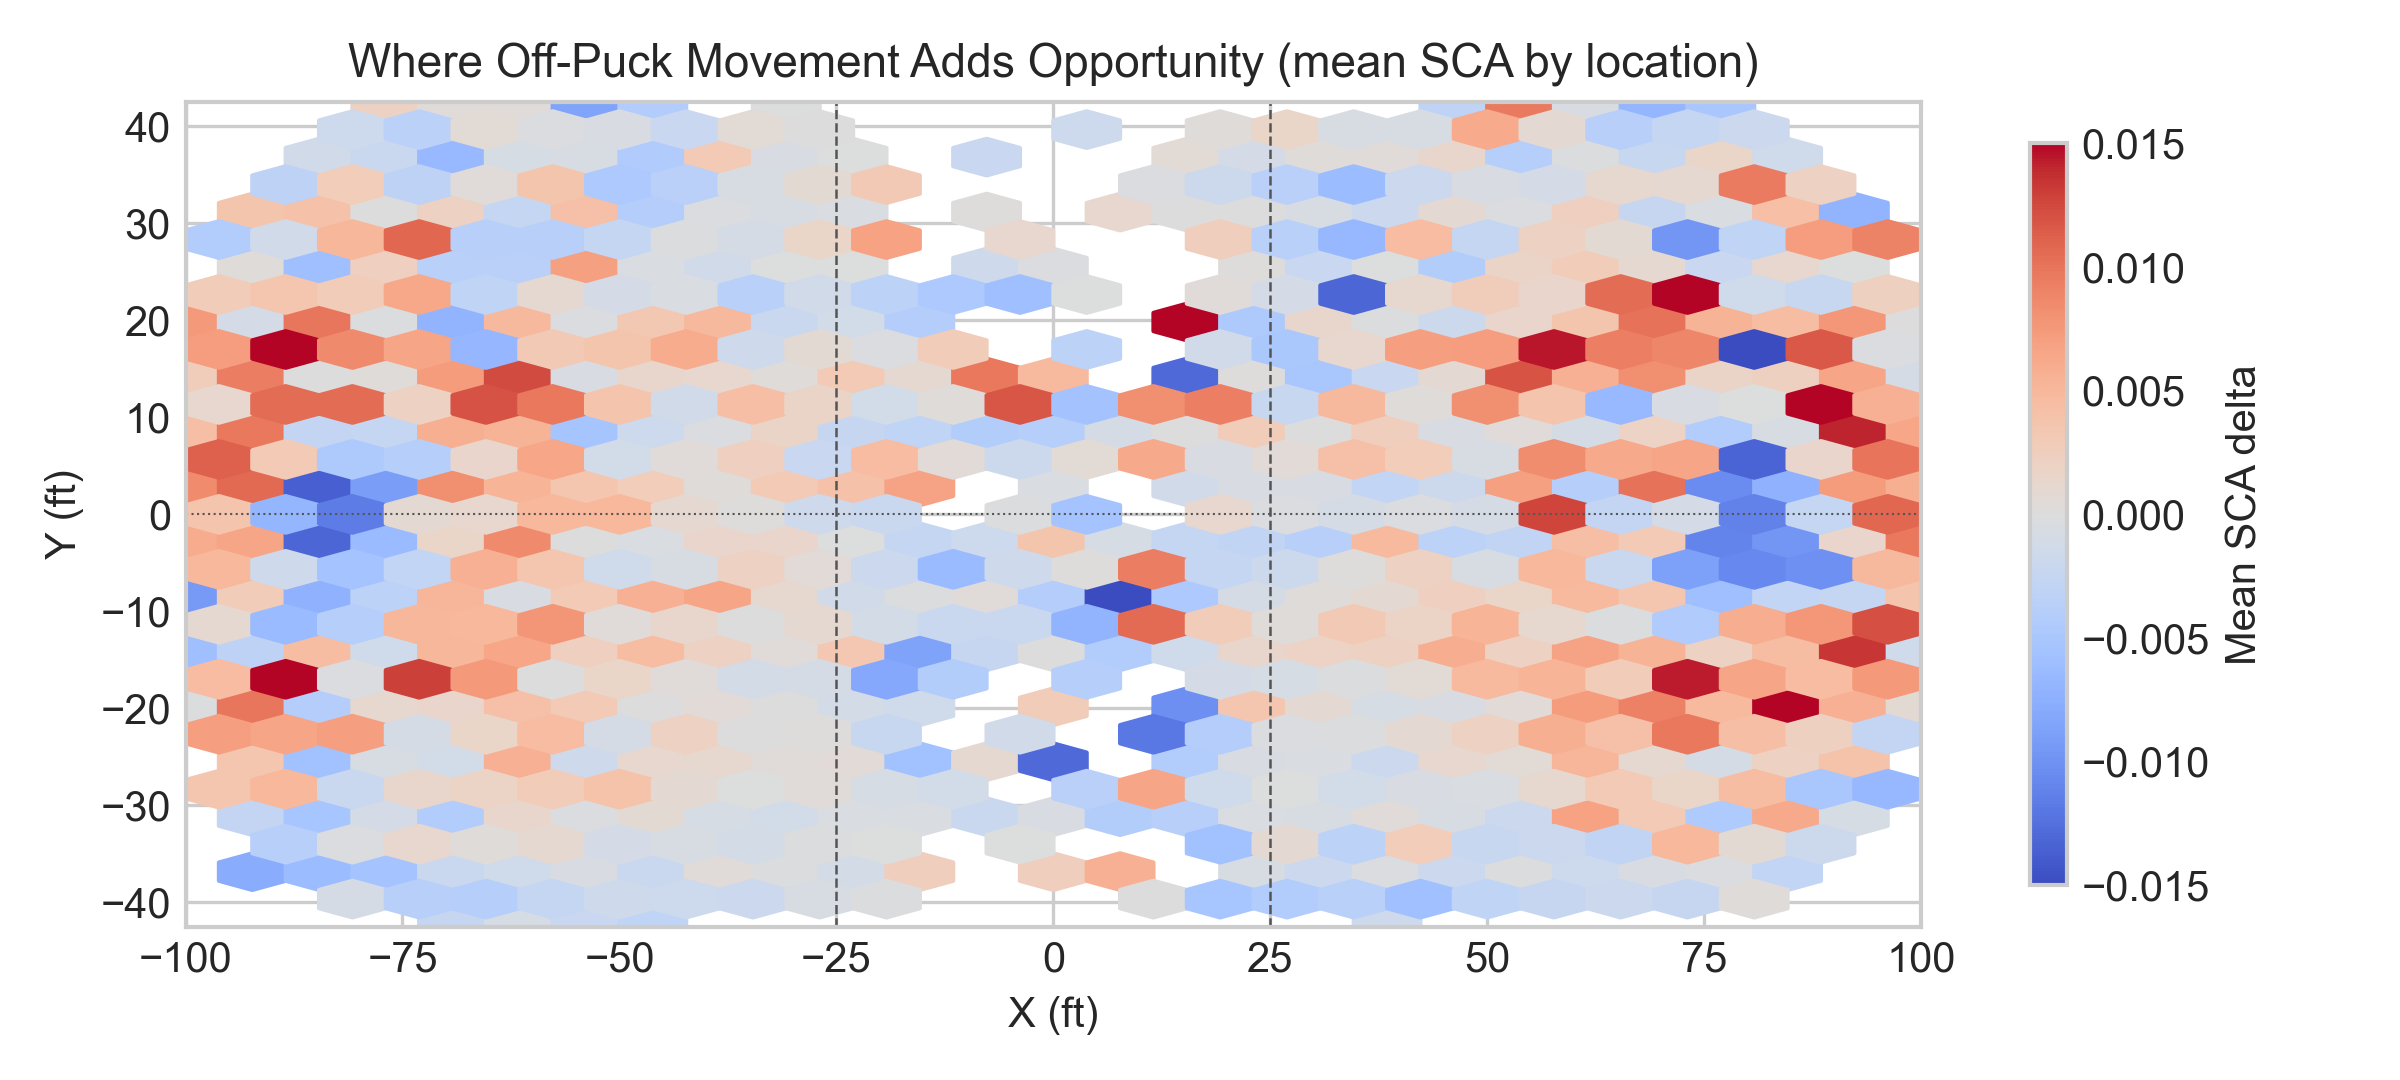
\includegraphics[width=\textwidth]{figures/fig_spatial_sca.png}
    \end{minipage}
    \caption{Player-level SCA leaderboard (min sampled frames threshold) and rink map of average SCA contribution by location.}
    \label{fig:leader_spatial}
\end{figure}

\section*{4. Limitations and Next Steps}
\begin{itemize}[leftmargin=1.2em,itemsep=0.2em]
    \item Current attribution uses freeze-based approximation, not full Shapley decomposition.
    \item Action detectors are rule-based and should be calibrated with manual video tags.
    \item Next revision: include teammate/opponent fixed effects and a stronger counterfactual defense assignment model.
\end{itemize}

\textbf{Code + data appendix path:} \texttt{projects/off\_puck\_space\_creation\_value/}

\end{document}

